\documentclass{beamer}
\usetheme{Berlin}
\usecolortheme{beaver}
\usefonttheme{serif}
\setbeamertemplate{navigation symbols}{}
\setbeamertemplate{caption}[numbered]
\setbeamercolor{section number projected}{bg=myred,fg=white}
\setbeamercolor{subsection number projected}{bg=myred,fg=white}
\setbeamertemplate{itemize item}{\color{myred}$\blacksquare$}
\setbeamertemplate{itemize subitem}{\color{myred}$\blacktriangleright$}

\usepackage{hyperref}
\usepackage[english]{babel}
\usepackage[utf8]{inputenc}
\usepackage{xcolor}
\usepackage{graphicx}
\usepackage{listings}

\title[]{Do ESG factors relate to yields of companies?}
\author{Gehrig, Li, Kuzmina, Zivanovic}
\titlegraphic{\centering
\includegraphics[width=2cm]{figures/uzh.png}}

\setbeamertemplate{footline} 
{
  \leavevmode%
  \hbox{%
  \begin{beamercolorbox}[wd=.333333\paperwidth,ht=2.25ex,dp=1ex,center]{author in head/foot}%
    \usebeamerfont{author in head/foot}\insertshortauthor%~~\beamer@ifempty{\insertshortinstitute}{}{(\insertshortinstitute)}
  \end{beamercolorbox}%
  \begin{beamercolorbox}[wd=.333333\paperwidth,ht=2.25ex,dp=1ex,center]{institute in head/foot}%
    \usebeamerfont{institute in head/foot}\insertshortinstitute
 \end{beamercolorbox}%
  
  \begin{beamercolorbox}[wd=.333333\paperwidth,ht=2.25ex,dp=1ex,right]{date in head/foot}%
    \usebeamerfont{date in head/foot}\insertshortdate{}\hspace*{2em}
    \insertframenumber{} / \inserttotalframenumber\hspace*{2ex} 
  \end{beamercolorbox}}%
  \vskip0pt%
}

\begin{document}

\begin{frame}
  \titlepage
\end{frame}

\begin{frame}{Contents}
  \tableofcontents
\end{frame}

\section{Introduction}
\begin{frame}{Introduction}
  \begin{itemize}
    \item Assessing factors introduced by Fama and French (1992).
    \item Focus on integrating ESG factors into factor models.
    \item \textbf{Research Question:} How do ESG factors relate to yields of companies?
  \end{itemize}
\end{frame}

\section{Factor Models and ESG in Existing Research}
\begin{frame}{Asset Pricing Models}
  \begin{itemize}
    \item \textbf{Efficient Market Hypothesis} by \textcite{Fama, 1970}: \\ All firm value information reflected in stock prices, complicating alpha generation.
    \item Introduction of the \textbf{Capital Asset Pricing Model (CAPM):}\\
    Systematic risk measurement through beta, leading to market risk assessment.
    \item Emergence of the \textbf{Arbitrage Pricing Theory:} \\
    Recognizing occasional market inefficiencies and short-term arbitrage opportunities.
  \end{itemize}
\end{frame}

\begin{frame}{Integration of ESG Factors}
  \begin{itemize}
    \item The Fama and French \textbf{Three Factor Model:} \\ Incorporating Small Minus Big (SMB) and High Minus Low (HML) into traditional market risk analysis.
    \item \textbf{Rise of ESG factors} in financial analysis: \\
     enhancing operational efficiency, stakeholder relations, and risk management.
    \item Correlation between strong ESG performance and higher company yields.
  \end{itemize}
\end{frame}



\section{Methodology}
\begin{frame}{Research Methodology}
  \begin{itemize}
    \item \textbf{Observation Period:} Data collected from September 1, 2014, to September 1, 2022.
    \item \textbf{Primary Focus:} Constituents of the Nasdaq 100 index.
    \item \textbf{Data Sources:}
      \begin{itemize}
        \item Nasdaq 100 constituents sourced from Wikipedia.
        \item Fama and French factors (1992) obtained as a CSV of monthly returns from their official website.
        \item Monthly returns and ESG scores fetched via Yahoo Finance.
      \end{itemize}
    \item \textbf{Data Cleaning Process:}
      \begin{itemize}
        \item Removal of columns with only NA (not available) values.
        \item Implementation of the fill-forward method for handling missing data.
      \end{itemize}
  \end{itemize}
\end{frame}

\section{Results}
\begin{frame}{Research Findings}
  \begin{itemize}
    \item Regression Analysis:
      \begin{itemize}
        \item All betas for \textcite{FamaFrench1992} factors are negative.
        \item Negative slope for market risk premium, challenging the concept of a reward for systematic risk.
        \item Negative coefficients for SMB and HML suggest favoring large firms and growth stocks.
      \end{itemize}
    \item Significance and Cautions:
      \begin{itemize}
        \item None of the t-values reach statistical significance at the 5\% level.
        \item Results should be interpreted cautiously due to lack of statistical significance.
      \end{itemize}
  \end{itemize}
\end{frame}

\begin{frame}{Results for \textbf{Four Factor Model}}
  \begin{figure}
    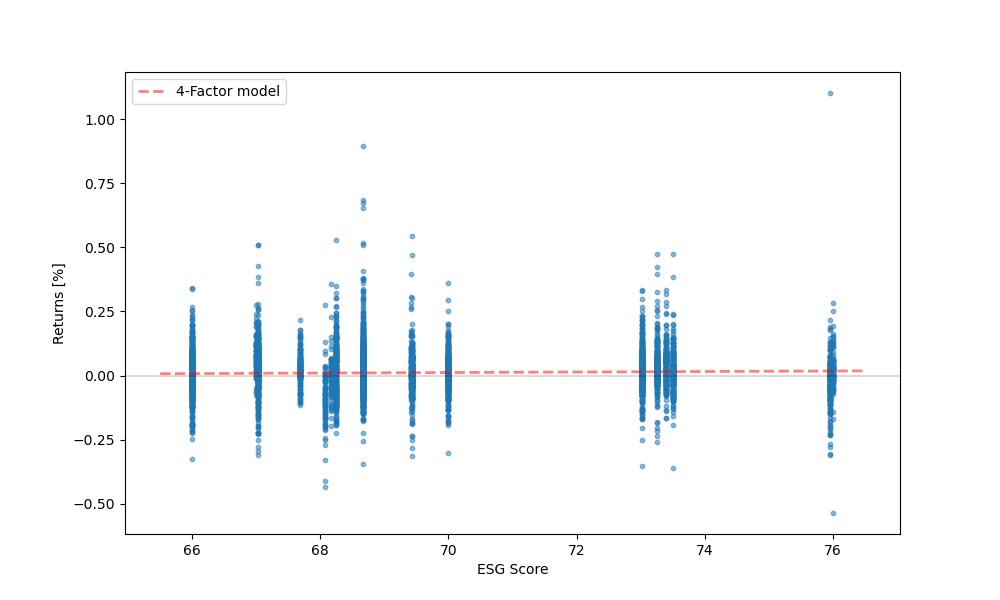
\includegraphics[width=0.65\textwidth]{figures/regression.png}
    \centering
  \end{figure}
      \begin{itemize}
        \item ESG factor shows a positive coefficient, indicating potential for higher yields with strong ESG scores.
        \item Lack of statistical significance for ESG factor under the 5\% level.
      \end{itemize}
\end{frame}

\section{Conclusion}
\begin{frame}{Conclusion}
  \begin{itemize}
    \item ESG factors can potentially lead to better yields.
\item Suggestions for Future Research:
      \begin{itemize}
        \item Extend the observation period and increase sample size for potentially higher statistical significance.
        \item Explore the possibility of a more robust relationship between ESG factors and company yields.
        \end{itemize}
  \end{itemize}
\end{frame}

\end{document}